% !TEX encoding = UTF-8 Unicode
\documentclass[fontsize=11pt,paper=a4,titlepage,DIV=calc,draft=false]{scrreprt}
% 11pt: Normale Textkörpergröße
% a4paper: Größe des Druckmediums
% titlepage: Titel auf einer separaten Seite ohne Seitenzahl
% twoside: Zweiseitiges Layout
% openright: Kapitel beginnen immer auf der rechten Seite
% headsepline: Trennt Textkörper von Headings durch Strich (entspr.: /footsepline)
% headinclude,footinclude: Kopf- und Fußzeile zählen zum Textkörper
% DIV=calc: Für die gewählten Optionen wird ein optimales Seitenverhältnis errechnet
% draft=true: Für Bilder wird die Box freigehalten, erheblicher Geschwindigkeitsvorteil.
% abstract: Setzt den Titel 'Zusammenfassung' vor den abstract

\usepackage{hyperref}

\usepackage{testcase}

\usepackage{upgreek}
%\usepackage{subfigure}

%  %  %  %  Bindungskorrektour  %  %  %  %
% \KOMAoptions{BCOR=10mm}

%  %  %  %  Abkürzungen  %  %  %  %
% Das Einführen dieser Befehler verhindert Umbrüche bei mehrgliedrigen Abkürzungen
\usepackage{xspace}
\newcommand{\zB}{\mbox{z.\,B.}\xspace}
% Abkürzung für zum Beispiel


%  %  %  %  Einheiten  %  %  %  %
%\usepackage[thinspace,thinqspace,squaren,textstyle]{SIunits}
% Komfoatables Paket zum Einbinden von Einheiten


%  %  %  %  Kodierung, Schrift und Sprache  %  %  %  %
\usepackage[utf8]{inputenc}
\usepackage{palatino}
\usepackage[ngerman]{babel}
% damit man Text aus dem PDF korrekt rauskopieren kann


%  %  %  %  Grafiken, Tabellen, Mathematikumgebungen  %  %  %  %
\usepackage{graphicx}
\usepackage{tabularx}
\usepackage{xcolor}
\definecolor{halfgray}{gray}{0.55}
\usepackage{amsmath,amsfonts,amssymb}
\usepackage{flafter,afterpage}
\usepackage[section]{placeins}
\usepackage{setspace} \onehalfspacing
\usepackage[margin=8mm,font=small,labelfont=bf,format=plain]{caption}
\usepackage[margin=8mm,font=small,labelfont=bf,format=plain]{subcaption}

\numberwithin{equation}{chapter}
\numberwithin{figure}{chapter}
\numberwithin{table}{chapter}


%  %  %  %  Kopf- und Fußzeilen  %  %  %  %

% \renewcommand\frontmatter{\pagenumbering{Roman}}
\usepackage{chngcntr}
\counterwithout{footnote}{chapter}

% Zeilenabstand zwischen zwei Fußnoten:
\footnotesep 9pt
% Einrücken der Fußnoten:
\deffootnote[1.5em]{1em}{1.5em}{\thefootnotemark\ \ }
%
%\usepackage{fancyhdr}				% Paket für leicht konfigurierbare Kopf- und Fußzeilen
%\fancypagestyle{plain}{				% Neue Gestaltung der Chapter- Page
%\fancyhf{} 							% Clear all header and footer fields
%\renewcommand{\headrulewidth}{0pt}		% Keine Trennlinie zwischen Kopf- / Fußzeile und Textkörper
%\renewcommand{\footrulewidth}{0pt}}
%
%\fancypagestyle{myfoot}{				% Neue Gestaltung der frontmatter pages
%\fancyhf{}							% Clear all header and footer fields
%\fancyhead[RO]{\thepage}				% Seitenzahl außen auf ungeraden Seiten
%\fancyhead[LE]{\thepage}				% Seitenzahl außen auf geraden Seiten
%\renewcommand{\headrulerwidth}{0pt}	% Keine Trennlinie zwischen Kopf- / Fußzeile und Textkörper
%\renewcommand{\footrulerwidth}{0pt}}
%
%\pagestyle{fancy}					% Pagestyle fancy aktiviert selbstkonfigurierten Style
%\fancyhf{} 							% Alle Kopf- und Fußzeilenfelder werden zunächst bereinig
%\renewcommand{\headrulewidth}{0pt}		% Keine Trennlienie zwischen Kopfzeile und Textkörper
%
%%\renewcommand{\chaptermark}[1]{\markboth{#1}{}}
%%\renewcommand{\sectionmark}[1]{\markright{#1}{}}
%
%\fancyhead[RO]{\leftmark ~~~~ \thepage}
%\fancyhead[LE]{\thepage ~~~~ \nouppercase \rightmark}


%  %  %  %  Überschriften  %  %  %  %


%  %  %  %  Verzeichnisse  %  %  %  %

% % % Literaturverzeichnis % % %
%\usepackage{natbib}

% % % Inhaltsverzeichnis % % %
% Die Chaptereinträge:
\usepackage{titletoc}

\titlecontents{chapter}
	[0pc]
	{
		\addvspace{0.5pc}
		%\filouter}
	}
	{\sffamily\Large\thecontentslabel\quad\sffamily\Large}{}
	{\titlerule*[0.75pc]{}\enskip\rmfamily\Large \contentspage}  % Wäre mit Seitenzahl 																					rechtsbündig
	[\addvspace{.5pc}]

% Die Sectioneinträge:
\titlecontents{section}
	[3.78em]
	{}
	{\rmfamily\contentslabel{2.3em}\rmfamily}
	{\hspace*{-2.3em}}
	{\titlerule*[0.75pc]{.}\enskip\contentspage}
	[\addvspace{.1em}]

% Die Subsectioneinträge:
\titlecontents{subsection}
	[6.2em]
	{}
	{\rmfamily\contentslabel{2.3em}\rmfamily}
	{\hspace*{-2.3em}}
	{\titlerule*[0.75pc]{.}\enskip\contentspage}
	[\addvspace{.1em}]

%\titlecontents{subsection}
	%[6.8em]
	%{}
	%{\rmfamily\normalsize\contentslabel{3em}\rmfamily\large}
	%{\hspace*{-2.3em}}
	%{\titlerule*[0.75pc]{.}\enskip\contentspage}

% Glossar einbinden und Abkürziungsverzeichnis erstellen
\usepackage[acronym,toc,section=section,numberedsection,nonumberlist]{glossaries}
\loadglsentries{./glossar}
\makeglossaries
\makeindex

% Zähler für Parts zurücksetzen
\makeatletter
\@addtoreset{chapter}{part}
\makeatother

\usepackage{todonotes}
\usepackage{listings}
\lstset{basicstyle=\ttfamily\normalsize,breaklines=true}


\begin{document}
\deftranslation[to=German]{Acronyms}{Abkürzungsverzeichnis}
%  %  %  %  Titelseite  %  %  %  %
\begin{titlepage}
	\vspace*{\fill}

	\rule{\textwidth}{0.25pt}

	\vspace*{1cm}

	\begin{singlespace}
		\begin{center}	\Large	\bfseries
			Software Engineering 2
		\end{center}
	\end{singlespace}

	\vspace{1em}

	\begin{singlespace}
		\begin{center}	\Large \bfseries
		Projektdokumentation
		
		\vspace{2em}	\large
		Projekt:
		
		Entwicklung eines Software-Systems
		
		zur Simulation der Steuerung eines Fahrstuhls
		\end{center}
	\end{singlespace}

	\vspace*{5cm}

	\rule{\textwidth}{0.25pt}

	\vspace*{\fill}
\end{titlepage}

%  %  %  %  Inhaltsverzeichnis  %  %  %  %

\tableofcontents

%  %  %  %  Hauptteil  %  %  %  %
%% \mainmatter
\chapter{Einführung}
\paragraph{}
Im Rahmen der Belegarbeit im Modul \textsc{Software Engineering 2} war ein Software-System zu implementieren, welches die Steuerung eines Fahrstuhls simuliert. Dieses Software-System soll in der Zukunft als Anschauungsmaterial im Lehrbetrieb verwendet werden. Studierenden soll damit ermöglicht werden, die Zusammenhänge zwischen real existierenden Automaten und der Thematik der Zustandsdiagramme zu erfahren.
\\
Die Dokumentation des Projektes gliedert sich in folgende Teildokumentationen:
\subsubsection*{Benutzerhandbuch}
Im Benutzerhandbuch werden Anweisungen für die korrekte Verwendung der Software gegeben. Sie kann Mitarbeitern oder Studierenden zur Verfügung gestellt werden, welche die Anwendung verwenden möchten. Neben den Hinweisen zur Verwendung sind die Systemvoraussetzungen sowie Installationsanweisungen enthalten.

\subsubsection*{Entwicklerhandbuch}
Um Eine Weiterentwicklung der Anwendung zu ermöglichen werden im Entwicklerhandbuch die internen Zusammenhänge und Strukturen dokumentiert. Enthalten sind die Klassendiagramme, sowie die Auflistung der Funktionen der \acrshort{API}.\\

\subsubsection*{Projektdokumentation}
Dieser Teil der Dokumentation wird sich mit Organisation der Projektarbeit beschäftigen. Analysiert werden die Herangehensweisen, verwendete Werkzeuge und verschiedene Entscheidungen die während der Projektarbeit getroffen worden. Ziel ist es die Zusammenarbeit und die Projektrealisierung zu reflektieren und entsprechende Schlüsse zu ziehen.

Ebenfalls behandelt dieser Abschnitt Themen der Analyse, der Qualitäts"-sicherung und des Software-Test.

\subsection*{Konventionen}
Folgende Konventionen werden im Dokument verwendet:\\
\begin{itemize}
	\item das entwickelte Software-System wird im folgenden Fahrstuhlsimulation genannt.
	\item Ordnernamen und Pfadangaben, sowie Codeausschnitte im laufenden Text sind durch eine nichtproportionale Schriftart gekennzeichnet
	\item Abkürzung werden nur bei der ersten Verwendung näher beschrieben, danach können sie zusätzlich im Glossar nachgeschlagen werden.
	\item Als Auftraggeberin wirkte Frau Professor Hauptmann, im folgenden als Kundin bezeichnet.
\end{itemize}

\part{Benutzerhandbuch}
\todo{kleine Einleitung}
\chapter{Systemvoraussetzungen}
\chapter{Installation}
\chapter{Anwendung}
\part{Entwicklerhandbuch}

\chapter{Übersicht}
\section{Technologien und Werkzeuge}
Um die Anforderungen an das Software-Projekt bestmöglich zu erfüllen werden verschiedene Web-Technologien und -Werkzeuge zur Umsetzung des Projektes verwendet. Im folgenden wird erläutert, an welcher Stelle des Projektes diese eingesetzt werden und warum.

\paragraph{Javascript}
Die Skriptsprache \textit{Javascript} wird im vorliegenden Projekt als Programmiersprache verwendet.
Der aktuelle \textbf{ECMA-262}\footnote{\url{http://www.ecma-international.org/publications/standards/Ecma-262.htm}} Standard, welcher im Allgemeinen als \textit{ECMAScript 6} bezeichnet wird, ermöglichte hierbei eine objektorientierte Implementierung.

\paragraph{node.js}
Um die Ausführung von Javascript-Code außerhalb eines Browsers zu ermöglichen wird die Laufzeitumgebung \textit{node.js} verwendet.

\paragraph{React.js}
Durch die Nutzung des Javascript-Frameworks \textit{React.js} ist es mög"-lich die Benutzerschnittstelle mit einem geringstmöglichen Aufwand zu implementieren und besonders effizient zu rendern.
Es wird hierbei der spezielle React-Syntax \textit{JSX} verwendet und mit sogenannten \textit{React-Komponenten} gearbeitet.
Diese Komponenten stellen dem Framework einen minimalen Satz an UI-relevanten Informationen bereit, welches dieses aufbereitet und somit in der Lage ist bei Änderungen ausschließlich jene Bereich erneuern, deren Daten sich tatsächlich verändert haben.

\paragraph{npm}
Um die Erfüllung von Abhängigkeiten im Laufe der Implementierung elegant und automatisiert zu gewährleisten wird die Javascript-Paketver"-waltung \textit{npm} genutzt.
Diese wird über die Datei \texttt{package.json} im Root-Verzeich"-nis der Anwendung konfiguriert.

\paragraph{bower}
Während \textit{npm} vorrangig Backend-relevante Pakete verwaltet, ist die Paketverwaltung \textit{bower} auf Frontend-spezifische spezialisiert.
So wird bower beispielsweise verwendet um Pakete wie \textit{bootstrap} oder \textit{React.js} einzubinden.
Die Konfiguration findet hier ähnlich zu \textit{npm} über eine Kon"-fi"-gu"-ra"-tionsdatei (\texttt{bower.json}) statt.

\paragraph{grunt}
Bei der Implementierung der Anwendungen wird \textit{ECMAScript 6}, sowie \textit{LESS} zur Beschreibung der Styles benutzt.
Selbst moderne Browser unterstützen dieses Technologien jedoch nur bedingt, weshalb verschiedene sogenannte Transpiler notwendig sind.
Diese und weitere Aufgaben werden mit Hilfe des \textit{grunt}-Frameworks verwaltet und automatisiert durchgeführt.
Die Datei \texttt{Gruntfile.js} enthält hierbei die Konfiguration der Tools.

\paragraph{karma \& jasmine}
Neben manuellen Software-Tests wurden im Rahmen des Projektes ebenfalls automatisierte Testverfahren entworfen und angewendet.
Eine Kombination der Frameworks \textit{karma} und \textit{jasmine} bilden hierzu die Grundlage.


\section{Systemvoraussetzungen}
Neben einem beliebigem Texteditor benötigt man zur Weiterentwicklung der Anwendung zunächst eine \textit{node.js}-kompatible Laufzeitumgebung. Diese kann z.B. unter \url{https://iojs.org/} für verschiedene Plattformen bezogen werden.

\paragraph{}
Nach der Installation von \textit{node.js} können alle weiteren Pakete und Werkzeuge mit Hilfe der Paketverwaltung \textit{npm} nachgeladen werden.
Diese ist Teil der \textit{node.js}-Installation. Um diese zu tun sind die folgende Befehle in einer Kommandozeile einzugeben:
\begin{lstlisting}
	npm install -g grunt
	npm install -g bower
	npm install
	bower install
\end{lstlisting}

Nach der Installation dieser Pakete sind alle Systemvoraussetzungen für Weiterentwicklung dieser Anwendung erfüllt.

\section{Build-Prozess}
Wie bereits mehrfach erwähnt war die große Kompatibilität zu verschiedenen Plattformen ein Grund für die Entscheidung, das Projekt mit Web-Tech"-no"-lo"-gien umzusetzen.
Als \textit{Build-Prozess} wird in diesem Kontext die Routine bezeichnet, die aus dem Quellcode des Projektes die Pakete erzeugt, welche an Kunden und Benutzer ausgeliefert werden.

\paragraph{}
Der \textit{Build-Prozess} wurde im vorliegenden Projekt mit Hilfe des \textit{grunt}-Frame"-works automatisiert und soll im folgenden beschrieben werden.
Diese Beschreibung eignet sich zusätzlich als Einführung in die Arbeitsweise des \glqq Task-Runners \grqq \textit{grunt}. Dargestellte Listings sind der \textit{grunt}-Kon"-fi"-gurations"-datei \\\texttt{Gruntfile.js} entnommen.

\begin{lstlisting}[language=JavaScript,label=JS:grunt_build,caption=grunt build-Task]
grunt.registerTask('build', function (target) {
	grunt.task.run([
		'dist',
		'nodewebkit',
	]);
});
\end{lstlisting}

Zeile 1 im Listing \ref{JS:grunt_build} zeigt die \glqq Anmeldung\grqq des Tasks im Framework.
Dies hat zur Folge das der beschriebene Task im Wurzelverzeichnis der Anwendung durch Eingabe des folgenden Befehls in einer Kommandozeile \texttt{grunt serve} ausgeführt werden kann.
Dieser Task bündelt nun die Ausführung von \texttt{dist} und \texttt{nodewebkit}.

\newpage
\begin{lstlisting}[language=JavaScript,label=JS:grunt_dist,caption=grunt dist-Task]
grunt.registerTask('dist', function (target) {
	grunt.task.run([
		'clean:dist',
		'useminPrepare',
		'concurrent:dist',
		'postcss',
		'concat',
		'cssmin',
		'uglify',
		'copy:dist',
		'filerev',
		'usemin',
		'htmlmin',
	]);
});
\end{lstlisting}

\paragraph{}
Listing \ref{JS:grunt_dist} zeigt den Inhalt des \textit{dist}-Tasks.
Die einzelnen Punkte entsprechen wiederum verschiedenen Unteraufgaben, welche in Tabelle \ref{dist_table} näher beschrieben sind.

\paragraph{}
Diese Aufgaben dienen alle der Vorbereitung des Quellcodes um im Anschluss mittels \texttt{nodewebkit} die fertigen Anwendungen zu erstellen.
Listing \ref{JS:grunt_webkit_config} zeigt die Konfiguration der entsprechenden Aufgaben.
Neben Quell- und Zielordner sind hier die jeweiligen Zielarchitekturen eingetragen.

\begin{tabularx}{0.92\textwidth}{lX}
	\textit{clean:dist} & löscht temporäre, sowie den dist-Ordner\\ \hline
	\textit{useminPrepare} & analysiert index.html auf Anweisungen welche Dateien mit usemin optimiert werden sollen\\ \hline
	\textit{concurrent:dist} & führt Unteraufgaben parallel aus um den Build-Prozess zu beschleunigen\\ \hline
	\textit{postcss} & analysiert CSS Code und fügt automatisch Anweisungen ein um die Kompatibilität mit älteren Browsern zu gewährleisten\\ \hline
	\textit{concat} & verknüpft mehrere Dateien zu Einer\\ \hline
	\textit{cssmin} & optimiert CSS-Dateien\\ \hline
	\textit{uglify} & optimiert Javascript-Dateien\\ \hline
	\textit{copy:dist} & Kopiert alle übrigen Dateien in den dist-Ordner\\ \hline
	\textit{filerev} & randomisiert Dateinamen um Probleme mit dem Cache des Browser zu vermeiden\\ \hline
	\textit{usemin} & führt die obigen Optimierungen automatisch basierend auf Anweisungen in index.html aus\\ \hline
	\textit{htmlmin} & verringert die Größe von HTML-Dateien\\ \hline
\end{tabularx}
\label{dist_table}
\vspace*{1cm}

\begin{lstlisting}[language=JavaScript,label=JS:grunt_webkit_config,caption=grunt nodewebkit-Konfiguration]
nodewebkit: {
	options: {
		platforms: [
			'win32',
			'win64',
			'linux32',
			'linux64',
			'osx64',
		],
		buildDir: 'builds',
	},
	src: ['dist/**/*'],
},
\end{lstlisting}

\paragraph{}
Nach Abschluss dieses Tasks befinden sich die Versionen zur Veröffentlichung in Unterordnern \texttt{ win32, win64, linux32, linux64} und\texttt{ osx64 }des Ordners \texttt{ dist } im Wurzelverzeichnis der Anwendung.

\chapter{Software-Entwurf}
\section{Grobentwurf}
Eine Prämisse des Projektes war stets den Fahrstuhl inklusive Steuerung mög"-lichst realitätsnah zu simulieren. Daher wurde die Anwendung von Beginn an in Teilsysteme untergliedert.

\paragraph{Komponentenstrukt}
Dies zeichnet sich insbesondere in der Struktur der Anwendung aus, welche aus mehrere Komponenten besteht, die wiederum in der Realität existierende Teilsysteme eines Fahrstuhlsystems abbilden.
So unterteilt sich das Gesamtsystem \textbf{Fahrstuhlsimulation} zunächst in die Teilsysteme \textbf{Fahrstuhlsteuerung} und \textbf{Visualisierung}, welche weiterhin verschiedene Komponenten beinhalten.

\paragraph{}
Im Entwurf der \textbf{Fahrstuhlsteuerung} sind dementsprechend \textit{Steuerung}, \textit{Sensoren} und \textit{Schnittstellen zur Passagierinteraktion} in voneinander unabhängige Komponenten gekapselt, welche sich im Feinentwurf auch als Klassen des Software-Systems wiederfinden.

\paragraph{}
Zu den Sensoren der Fahrstuhlsimulation gehören \textit{Etagen-}, \textit{Tür-}, und \textit{Gewichtssensoren}.
Deren Kommunikation mit der Steuerung erfolgt ebenfalls über definierte Schnittstellen, wobei zusätzlich zu unterscheiden ist, ob es sich um aktive oder Passive Sensoren handelt.

\paragraph{MVC-Paradigma}
Auf einer hohen Abstraktionsebene kann das System so auch unter dem MVC-Modell\footnote{Abk. für Model-View-Controler-Modell} betrachtet werden.
Die Intention besteht darin die Fahrstuhlsteuerung als Modell zu charakterisieren und die Kommunikation mit der Benutzerschnittstelle, der View, über einen Controller zu etablieren.
Somit Kommunizieren die verschiedenen Teilsysteme ausschließlich über definierte Schnittstellen und die Paradigmen Modularität und Wiederverwendbarkeit sind inhärent erfüllt.

\paragraph{Steuerungs-Algorithmus}
Neben der Struktur der Anwendung ist ebenfalls ein aus der Realität bekannter Algorithmus zur Steuerung des Fahrstuhls adaptiert worden, der sogenannte \textit{Fahrstuhl-Algorithmus mit Sammelsteuerung}\cite{wiki_elev}.
Dieser bedient zunächst Fahrtwünsche und -Rufe auf der aktuellen Fahrtrichtung und kehrt diese im Anschluss um.

\paragraph{}
Die Fahrstuhlsteuerung muss nun beim Erreichen einer Etage unter anderem zwei Fragen beantworten:

\begin{enumerate}
	\item Existiert ein Fahrtwunsch /-Ruf auf dieser Etage und muss dementsprechend angehalten werden?
	\item Existieren Fahrtwünsche /-Rufe ober- oder unterhalb der aktuellen Etage, beziehungsweise muss die Fahrtrichtung beibehalten oder umgekehrt werden?
\end{enumerate}

\paragraph{}
Frage 2. ist in dem Fall die interessantere.
Ein naiver Ansatz könnte folgendermaßen außen:\\ \\ Ein System besitzt $N$ Etagen, die Kabine befindet sich aktuell in Etage $M$ und fährt in Richtung $X$.
Um zu entscheiden ob die Fahrt in der aktuellen Fahrtrichtung fortgesetzt wird durchsucht die Steuerung die Datenstruktur der Etagen linear im Bereich $(M,N]$ für $X>0$ (aufwärts) oder im Bereich $[0,M)$ für $X<0$ (abwärts).\\\\
Dieser Algorithmus wäre jedoch abhängig von der Menge der Etagen und besäße damit die Komplexität $\mathcal{O}(n)$.

\paragraph{}
Beim Entwurf des Algorithmus der vorliegenden Anwendung war das Ziel diese Komplexität zu verringern.
Seine Funktion erklärt sich wie folgt:\\ \\ Grundlegendes Element des Algorithmus ist eine Datenstruktur, welche ausschließlich die \textbf{Summe} der Fahrtwünsche /-Rufe über- und unterhalb der aktuellen Position enthält.
Um nun über die Fahrtrichtung entscheiden zu können muss die Fahrstuhlsteuerung ausschließlich an definierten Stellen in dieser Datenstruktur überprüfen, ob Elemente größer 0 sind.
Die Komplexität dieser Abfrage über einer Datenstruktur fester Größe besitzt die Komplexität $\mathcal{O}(1)$, was einer Reduktion entspricht.
Zu beachten ist dabei jedoch, dass die genannte Datenstruktur zu jedem Zeitpunkt aktuell gehalten werden muss. Dies ist jedoch ein implementierungsspezifisches Problem, dessen Lösung in der Sektion \textit{\nameref{imp_model}} im Kapitel \textbf{\nameref{imp}} beschrieben wird.

\section{Feinentwurf}

\paragraph{React}
Wie bereits erwähnt wurde erleichtert das \textit{React}-Framework die Entwicklung performanter Webanwendungen.
Bei der bisher im Web üblichen Herangehensweise wurde in der Regel das HTML der Website Serverseitig gerendert.
Trat eine gewisse Änderung in dem Clientseitigen Model auf, z.B. weil dem Client vom Server neue Daten zugesendet wurden, so wurde \textit{explizit} der jeweilige Bereich der Seite, welcher diese Daten darstellte, erneuert.
Die einzigen zwei Möglichkeiten um dies zu erreichen, sind hierbei natürlich nur die, die jeweiligen \textit{explizit} Attribute einer \textit{DOM-Node}, wie z.B. Farbe, oder den Text, der Bereiche zu ändern, oder aber den gesamten Bereich in neuem HTML zu rendern.
Wie man sich leicht Denken kann, führt Ersteres eventuell zu der Frage, welcher Teil des Codes für was Verwantwortlich ist, oder aber erschwert die Entwicklung durch eine Überzahl an nötigen Controllern.
Letzteres wiederum ist eine eventuell äußerst inperformante Lösung, da das rendern von ganzen Bereichen der Seite auch jene betrifft die sich möglicherweise gar nicht geändert haben.

\paragraph{}Als zur Zeit noch äußerst moderne Lösung bietet sich hierfür das aufstrebende React Framework, welches seit seiner Veröffentlichung mit Worten wie \glqq Bahnbrechend\grqq und \glqq Revolutionär\grqq betitelt.
Hierbei schreibt der Entwickler sogenannte React-Komponenten.
Statt nun bei einem Render-Vorgang dem React Framework fertigen HTML Code zu liefern, den die jeweilige Komponente darstellen will, muss sie stattdessen eine ebenso hierarische Objektstruktur zurückgeben, welche \textit{repräsentativ} für den HTML Code steht.
Diese repräsentative Struktur ähnelt dem und simuliert den sogenannten \textit{Document Object Model} (DOM), weshalb man diese Struktur auch den \textit{Shadow DOM} nennt.
Bei jeder Änderung des Zustands einer Komponente wird hierbei nun die \textit{render}-Methode neu aufgerufen.
Ändert sich zwischen 2 Aufrufen der \textit{Shadow DOM}, so wird ein möglichst minimaler Satz an Modifikationen berechnet, welche nötig sind um den alten \textit{Shadow DOM} in den neuen zu transformieren.
Dieser Satz an Änderungen wird nun auf den tatsächlichen \textit{DOM} des Browsers angewendet. \\

Diese Vorgehensweise ist selbstverständlich nicht so performant wie eine optimale und explizite Verwaltung des HTML und des \textit{DOMs}, jedoch ist die Performanz für nahezu alle Einsatzgebiete bei weitem ausreichend.
Da die Komplexität bei größeren Projekten jedoch stark zunimmt und somit eine optimale und explizite Verwaltung exponentiell schwieriger wird, übersteigt die Performance einer Website die React verwendet meistens die einer ohne.
Zusätzlich eleminiert React die Frage gänzlich, wie und wo man Änderungen auf eine Website anwenden und verwalten kann und ermöglicht somit zu"-sätzlich eine äußerst schnelle Entwicklung.

\paragraph{Publish/Subscribe Pattern}
In der Web-Entwicklung ist zur Zeit eine Komponentenorientierte Entwicklung gebräuchlich, bei denen die Komponenten untereinander nur lose gekoppelt sind.
Um dies zu erreichen wird in der Regel das \textit{Publish/Subscribe} (PubSub) Pattern verwendet, welches dem traditionellen \textit{Observer} Pattern sehr ähnlich ist.
Statt sich als Objekt beim Subjekt explizit registrieren zu müssen, existiert hier ein Datenkanal welcher sogenannte \textit{Events} an alle \textit{Subscriber} verteilt.
Jedem Objekt steht es frei sich als \textit{Subscriber} bei diesem Kanal für einen bestimmten \textit{Event}-Typen ein- und auszutragen.
Des Weiteren existiert exakt ein Objekt welches als \textit{Publisher} fungiert und \textit{Events} eines bestimmten Typs mit einer beliebigen Anzahl an Parametern an alle Subscriber versenden kann.
Die Idee ist es hierbei also die einzelnen Klassen und Komponenten noch loser zu koppeln und stärker voneinander zu trennen, indem man selbst die letzten Abhängigkeiten zwischen Objekt und Subjekt, wie sie im klassischen Observer Pattern existieren, eleminiert.
Besonders mit Programmiersprachen wie ECMAScript lässt sich dies sehr leicht erzielen, da Funktionen hier nur eine spezielle Form von Objekten und sogenannte \textit{Lambda}-Funktionen sind.
Sie können sowohl eine beliebige Anzahl an Parametern annehmen, als auch mit einer beliebigen Anzahl aufgerufen werden.
Es ist somit möglich und üblich das PubSub Pattern mit \textit{Lambda}-Funktionen zu nutzen, um sowohl eine dynamische Menge an \textit{Event}-Typen und \textit{Event}-Parametern verarbeiten zu können, als auch eine vollständige Entkopplung zwischen \textit{Publisher} und \textit{Subscriber} zu erreichen.

\chapter{Implementierung}
\label{imp}

\paragraph{Klassendiagramm}
\begin{figure}[h!]
	\hspace*{-2cm}
	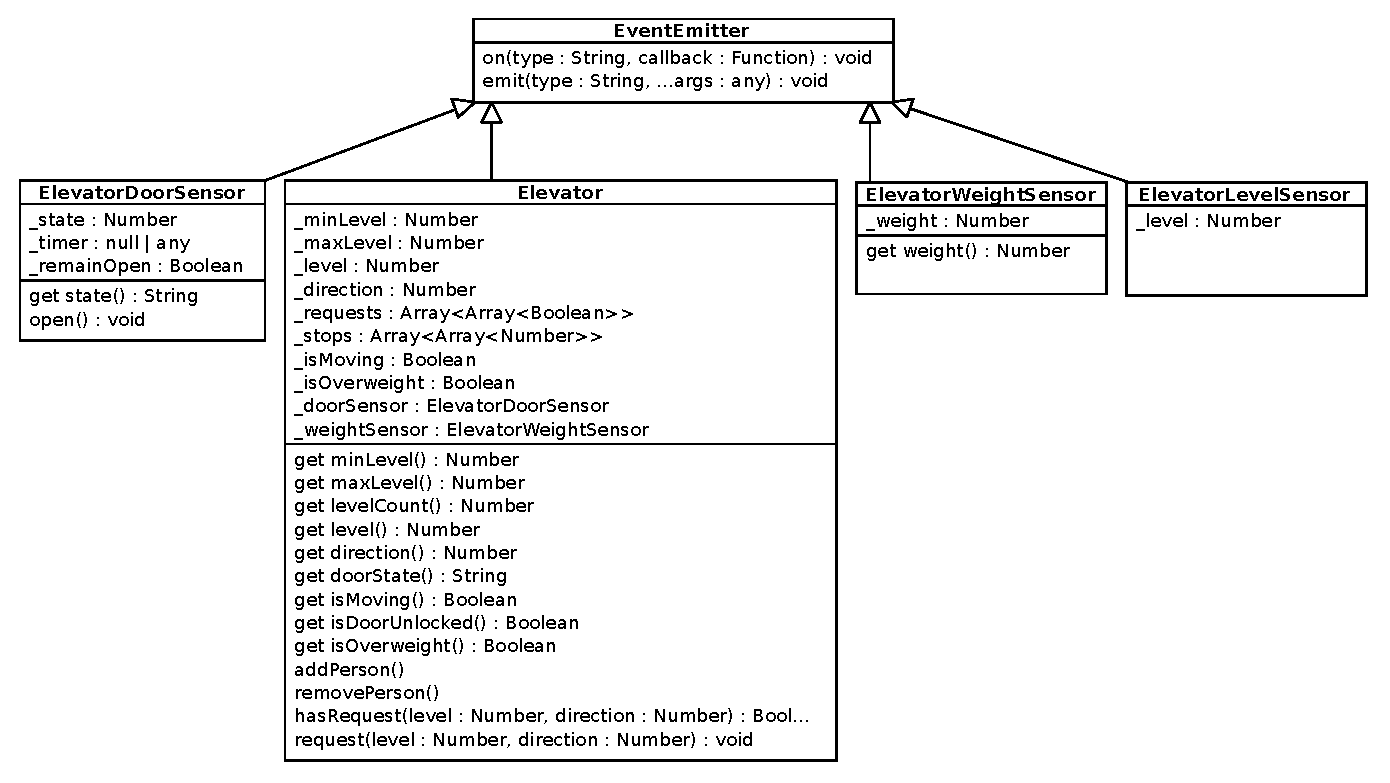
\includegraphics[width=1.3\textwidth]{images/klassendiagramm.eps}
	\caption{Übersicht der verwendeten Klassen der Hauptkomponente Fahrstuhlsteuerung}
	\label{klassdiagramm}
\end{figure}

\section{Model}
\label{imp_model}
Als zentraler Kern des Model steht die Klasse \texttt{Elevator}.
Dieser steht in Verbindung mit seinen 3 Sensor-Klassen \texttt{ElevatorDoorSensor}, \texttt{Elevator""LevelSensor} und \texttt{ElevatorWeightSensor}.
Des Weiteren wird die \texttt{Event""Emitter}-Klasse, welche das \textit{PubSub} Pattern implementiert und von \texttt{node.js}, bzw. von entsprechenden Shims für den Browser, zur Verfügung gestellt wird.
Wie im Entwurf bereits geplant wurde, sollen alle 4 \texttt{Elevator*} Klassen als möglichst eigenständige Komponenten existieren und erben deshalb alle von der \texttt{EventEmitter}-Klasse.
Während eine \texttt{Elevator}-Instanz also konstruiert wird, erstellt diese jeweils eine Instanz der 3 Sensor-Klassen und übergibt eine Referenz von sich selbst als Parameter.
Dadurch haben die Sensor-Klassen in ihren Konstruktoren Zeit sich beim \texttt{Elevator} als Subscriber für Events zu registrieren, die für sie relevant sind.
\textit{Keine} dieser Klassen hält jedoch eine explizite Referenz zum \texttt{Elevator} aufrecht, was die nötige Entkopplung für eine gute Komponentenarchitektur aufrecht erhält.
Der \texttt{Elevator} wiederum registriert sich selbst als Subscriber für die für ihn relevanten Events bei den Sensoren.
Der \texttt{Elevator} ist außerdem derjenige der eine Referenz zu den Instanzen der Sensorklassen aufrecht erhält --- man kann sagen, dass eine \texttt{Elevator}-Instanz \glqq Besitzer\grqq der Sensor-Instanzen ist.
Nahezu jegliche Kommunikation findet zwischen der Elevator-Instanz und einer Sensor-Instanz nun durch das \textit{PubSub} Pattern statt. \\

Die \texttt{Elevator}-Klasse, welche als \glqq Frontend\grqq des Models dient, stellt nun eine gewisse Zahl an öffentlichen Methoden zur Steuerung bereit, welche auch im Abschnitt \textit{\nameref{imp_api}} näher beleuchtet werden.
Die primäre Methode ist hierbei die \texttt{request}-Methode.
Wird versucht einen neuen Request hinzuzufügen, so wird dieser zunächst auf Validität geprüft.
Die überprüften Parameter sind die Etage zu der der \texttt{Elevator} fahren soll, als auch die ageforderte Richtung, welche als Integerwert übergeben muss.
Dieser Wert müssen wie auch an allen anderen Stellen die mit einer Fahrtrichtung arbeiten kleiner Null sein falls es ein Runter-, größer Null falls es ein Hoch- und gleich Null sein falls es ein Request vom Innentableau ist.
Ist er valide, so wird geprüft, ob sich der \texttt{Elevator} bereits auf der geforderten Etage befindet und still steht.
Sollte dies der Fall sein so wird nun die \texttt{open}-Methode des \texttt{ElevatorDoorSensor} aufgerufen.
Dies ist auch die zur Zeit einzige Verwendung eines direkten Methodenaufrufs im Model, da ansonten ein eigener Event-Typ einzig für diese eine Verwendung hätte hinzugefügt werden müssen und dies wäre nicht im Sinne des PubSub Patterns gewesen, welches eher auf eine 1:N-Verteilung abzielt.
Sollte dies alles jedoch nicht der Fall sein, so wird der Request dem \texttt{Elevator} hinzugefügt. \\

Die Requests werden hierbei in einem Array aus Boolean-Tripeln im Member \texttt{\_requests} registriert.
Jedes Tripel in diesem Array steht hierbei reprä"-sentativ für die noch ausstehenden Requests auf einer Etage entsprechend der Array-Position.
Hierbei, sowie in allen Weiteren Verwendungen von Tripeln in der \texttt{Elevator}-Klasse, ist das erste Element wahr falls auf der jeweiligen Etage ein Runter-Request aktiv ist.
Das zweite Element ist ebenfalls wahr falls ein Hoch-Request aktiv ist, sowie das dritte Element welches für einen Request aus dem Innentableau steht.
Des Weiteren existiert zusätzlich ein Tupel aus zwei gleichermaßen aufgebauten Integer-Tripeln, welches im Member \texttt{\_stops} gespeichert wird.
Das erstere Tripel \textit{zählt} hierbei, wie bereits erklärt wurde, die jeweiligen Summen aller aktiven Requests unter und das Zweitere respektive alle über der aktuellen \texttt{Elevator}-Position. \\

Sollte sich der Fahrstuhl nun aktuell noch im Idle-Zustand befinden, so kann mittels der \texttt{\_beginMoving}-Methode direkt in die entsprechende Richtung losgefahren werden.
Ist dies nicht der Fall und sind die Türen nicht verschlossen, so kommt der \texttt{Elevator}DoorSensor ins Spiel. \\

Der \texttt{Elevator}DoorSensor öffnet selbstverständlich die Türen sobald eine gewünschtes Ziel, bzw. ein Request, erreicht wird.
Dieses Ereignis wird vom \texttt{Elevator} mit dem \glqq stop\grqq-Event signalisiert und vom \texttt{ElevatorDoor""Sensor} aufgegriffen.
Dieser ruft nun seine \texttt{open}-Methode auf, welche eine interne State-Machine ins Rollen bringt, die die Zustände \textit{opening}, \textit{open}, \textit{shutting} und \textit{shut} abarbeitet.
Wie man bereits erkennen kann erfüllt der \texttt{Elevator""Door""Sensor} trotz seines Namens nicht nur eine reine passive Sensor-, sondern auch eine Simulationsfunktion.
Bei einem Aufruf der \texttt{open}-Methode, sowie wenn ein State erreicht wurde, wird dessen Zustandsname als gleichnamiges Event verteilt und der nächste State mittels simplen Timern angesetzt, sofern nicht bereits der \textit{shut}-Zustand erreicht wurde, oder aber der \texttt{\_remain""Open}-Member wahr ist.
Aufgrund der Implementierung des \texttt{ElevatorDoor""Sensor} als State-Machine, ist es in der Lage bei einem weiteren Aufruf der \texttt{open}-Methode die Timer zurückzusetzen, bzw. die Tür erneut zu öffnen, wäh"-rend sie aktuell offen ist, bzw. respektive während sie aktuell schließt. \\

Der \texttt{Elevator} greift hierbei nun das \textit{shut}-Event mit seiner \texttt{\_onDoorShut}-Methode als Callback auf und versucht daraufhin gleichermaßen wie in der \texttt{request}-Methode loszufahren.
Da nun jedoch die Türen geschlossen sind so kann im Gegensatz zu vorher losgefahren werden. \\

Fährt der \texttt{Elevator} von einer Etage aus los so fährt so wird mit einem \textit{move}-Event die aktuelle Etage und die Fahrtrichtung signalisiert.
Hierfür wird nun der \texttt{ElevatorLevelSensor} relevant. \\

Der \texttt{Elevator} erstellt selbstverständlich bei der Konstruierung für jede Etage einen eigenen \texttt{ElevatorLevelSensor}.
Jeder dieser Instanzen registriert sich selbst bei dem \texttt{Elevator} für \textit{move}-Events.
Wird eines ausgelöst so erhält nun jeder Sensor in der Simulation eine Nachricht und jeder prüft ob es der Sensor wäre der der nächstgelegenen Etage in der Fahrtrichtung entspricht.
Dieser Sensor setzt nun einen Timer auf, welcher nach einer festen Zeit ein \textit{contact}-Event auslöst. \\

Der \texttt{Elevator} wiederum registriert sich bei der Konstruierung mit seiner \texttt{\_onLevelContact}-Methode für die \textit{contact}-Events bei jedem \texttt{Elevator""Level""Sensor}.
Wird eines ausgelöst signalisiert dies dem \texttt{Elevator} den Kontakt, bzw. die Ankunft, bei einer Etage.
Diese Ankunft macht der \texttt{Elevator} nun publik indem er zunächst ein \textit{change:level}-Event auslöst.
Sollte des Weiteren auf der nun angekommenen Etage ein Request vorliegen so wird außerdem ein \textit{stop}-Event ausgelöst, der Request aus \texttt{\_requests} entfernt, sowie der entsprechende Eintrag in \texttt{\_stops} dekrementiert.
Dieses Event wird unter anderem vom \texttt{ElevatorDoorSensor} aufgegriffen, welcher dadurch die Türen öffnet.
Die \texttt{\_onLevelContact}-Methode implementiert hierbei außerdem das Kernstück des sogenannten Aufzug-Algorithmus.
Es wird also solange in die aktuelle Bewegungsrichtung weitergefahren bis keine Requests mehr in die Richtung vorliegen.
Ist dies der Fall so wird die Gegenrichtung geprüft und entsprechend die Richtung umgekehrt.
Sollte auch in der Gegenrichtung keine Requests vorliegen so wird ein \textit{idle}-Event ausgelöst.
\texttt{\_stops} hilft hierbei enorm, da auf Iterationen durch das Requests-Array verzichtet werden kann.
Sollte der Fahrstuhl jedoch weiterfahren, so muss nun das nächste \textit{move}-Event ausgelöst werden.
Bevor dies geschiet wird jedoch sichergestellt, dass wenn der Fahrstuhl einen Request in die entgegengesetzte Richtung überspringt, die entsprechenden Summen in \texttt{\_stops} angepasst werden, indem dessen gedachter Eintrag von der einen Seite des Fahrstuhls auf die anderen Seite über"-tragen wird. \\

Zuletzt existieren öffentliche APIs im \texttt{Elevator} um Personen hinzuzufügen, bzw. um sie zu entfernen.
Aufrufe dieser Methoden führen jeweils dazu, dass ein \textit{persons:add}-, bzw. respektive ein \textit{persons:remove}-Event ausgelöst wird.
Dieses Events werden vom \texttt{ElevatorWeightSensor} aufgegriffen, welcher sich bei seiner Konstruierung beim \texttt{Elevator} hierfür registriert, welche jeweils dazu führen, dass der \texttt{ElevatorWeightSensor} seinen Member \texttt{\_weight} um den fixen Wert des Gewichts einer Person vergrößert, bzw. verringert.
Wird das maximale Gewicht überschritten, oder aber wieder unterschritten nachdem das maximale Gewicht bereits erreicht wurde, so wird ein \textit{change}-Event ausgelöst, welches als einzigen Parameter übermittelt, ob der \texttt{Elevator""WeightSensor} aktuell Überlast, oder Normallast meldet. \\

Dieses Event wird hierbei vom \texttt{Elevator} wiederum aufgriffen, welcher den Zustand zwischenspeichert und als Mediator das Ereignis als \textit{overweight:""change}-Event weiterleitet.
Der \texttt{ElevatorDoorSensor} registriert sich beim \texttt{Elevator} nun außerdem in seinem Konstruktur für eben jenes Event, setzt seinen \texttt{\_remainOpen}-Member entsprechend und ruft die \texttt{open}-Methode auf.
Wie bereits erwähnt wurde sorgt nun ein Wahr-Wert im \texttt{\_remainOpen}-Mem"-ber dafür, dass \texttt{ElevatorDoorSensor} im \textit{open}-Zustand verbleibt.

\section{View/Controller}
\label{imp_vc}
Durch die Verwendung von React als Framework fallen View und Controller sehr schlank aus --- der Großteil des Codes ist hierfür nur zuständig sich für die entsprechenden Events zu registrieren und den HTML Code zu beschreiben.
Als Einstiegspunkt des gesamten Codes dient hierbei die \texttt{main.jsx} Datei, welche alle Weiteren React Komponenten in den statischen HTML Code der \texttt{index.html} einhängt.
Des Weiteren wird darin die Elevator-Instanz erstellt, welche den 3 folgenden Komponenten als statisches Property übergeben wird. \\

Die ElevatorView Komponente ist hierbei nun eine dieser Komponenten und auf der linken Seite der Website zu sehen.
Sie erstellt eine Instanz der ElevatorCarView Komponente und für jede Etage des Elevator eine Instanz der ElevatorLevelView Komponente.
Jeden dieser Instanzen wird wiederum die Elevator-Instanz als Property übergeben, sowie letzteren die Etagennummer für die sie stehen. \\

Die ElevatorCarView Komponente registriert sich hierbei für \textit{move}-, \textit{persons:add}-, \textit{persons:remove}-, \textit{door:open}- und \textit{door:shutting}-Events bei dem Elevator.
Das \textit{move}-Event wird hierbei verwendet um eine vertikale Animation der ElevatorCarView innerhalb der ElevatorView zu der Höhe der entsprechenden ElevatorLevelView vorzunehmen.
Die \textit{persons:}-Events werden des Weiteren dafür verwendet um die Personenanzahl aktuell zu halten, sowie die \textit{door:}-Events dafür verwendet werden um bei geöffneten Türen die Buttons zum ändern der Personenanzahl verfügbar zu machen.
Wird einer dieser Buttons gedrückt so propagieren die entsprechend \textit{click}-Events durch den \textit{DOM} des Browsers zu den Handlern des React Frameworks welche die Komponente darüber informieren.
Diese ruft daraufhin die entsprechende \texttt{addPerson}-, bzw. \texttt{removePerson}-Methode auf. \\

\newpage
Die ElevatorLevelView Komponente registriert sich ebenfalls für die \textit{door:""opening}-, sowie \textit{door:shutting}-Events, aber auch für die \textit{requests:add}-, \textit{requests:""remove}-Events.
Erstere werden dafür verwendet um die Türen öffnend, bzw. schließend zu animieren.
Letzere hingegen werden dafür verwendet um bei Änderungen des \texttt{\_requests}-Members des Elevator die entsprechenden Hoch- und Runter-Buttons mit einer grünen Farbe signalisieren zu lassen, dass sie aktiv sind und für sie ein Fahrtwunsch bereit liegt.
Entsprechend der vorhergehenden Komponente werden bei einem druck auf die Buttons die \texttt{request}-Methode des Elevator aufgerufen. \\

Neben der ElevatorView existiert jedoch außerdem die AccessoryView.
Diese registriert sich für die \textit{change:level}- und \textit{change:overweight}-Events beim Elevator.
Das Erstere wird dafür verwendet, um die Anzeige der aktuellen Etage auf den neuesten Stand zu halten.
Letzeres hingegen dient zur Anzeige des Fahrstuhlzustands, sprich: Normalzustand, oder Überlast.
Außerdem bindet die AccessoryView das AccessoryPanel ein, dessen \texttt{show}-Methode bei einem \textit{mouseenter}-Event des Browsers aufgerufen wird.

\paragraph{}
Das AccessoryPanel ist eine Komponente die das Innentableau darstellen soll.
Dieses registriert sich ebenfalls für die \textit{requests:add}-, \textit{requests:remove}-Events um bei Änderungen im Elevator die entsprechenden Buttons aktiviert darzustellen.
Um den Inhalt als schwebendes Panel darzustellen wird die Popover Bibliothek von \textit{Bootstrap} verwendet.
Auch hier wird bei einem druck auf einen der Buttons die \texttt{request}-Methode des Elevator direkt aufgerufen.

\paragraph{}
Zu guter Letzt existiert die UmlView-Komponente.
Diese Komponente verwendet jedoch als einzige keinerlei interaktive Features.
Stattdessen lädt sie mittels einem XMLHttpRequest das UML Diagramm von \texttt{images/uml.svg}, fügt es als eigenen HTML-Content ein und registriert sich bei dem Elevator für alle für das Zustandsdiagramm relevanten Events.
Als primäre Methode um einen Zustand im Diagramm zu markieren wird \texttt{pushActive} verwendet, welcher die IDs von den Zuständen im SVG-Code übergeben und deren DOM Node in einem Array hinterlegt.
Diese implementiert einen einfachen FIFO Algorithmus bei dem die Elemente in den Positionen 0 bis 2 jeweils die CSS Klasse \texttt{.active-0} bis \texttt{.active-2} zugewiesen bekommen.
Hierbei wird jedoch nur dann das erste Element entfernt wenn auch mindestens ein Zweites existiert.
Des Weiteren wird auch nur mindestens alle 333ms das erste Element entfernt.
Dies stellt sicher, dass auch Zustände welche keine Verweildauer haben, wie z.B. der Übergang von \glqq Fahre hoch\grqq in \glqq Fuhr hoch\grqq, welches instant direkt in z.B. \glqq Tür öffnet sich\grqq übergeht, für den Anwender wahrnehmbar sind.

\newpage
\section{Benutzerschnittstelle}
Damit die aktiven Zustände hervorgehoben werden können, müssen sie eindeutig identifizierbar sein.
Dafür wurden die Elemente der Grafik gruppiert und mit IDs versehen, auf die mittels Javascript und dem \acrshort{DOM} zugegriffen werden kann.
Abbildung \ref{fig:ZD_id_view} stellt die Identifikatoren dar.
Bei der Benennung der IDs wurden folgende Konventionen angwendet:
\begin{itemize}
	\item präfix uml- für alle Bezeichner
	\item Worte durch Bindestriche getrennt
\end{itemize}

\begin{figure}[hbt]
	\hspace*{-2cm}
	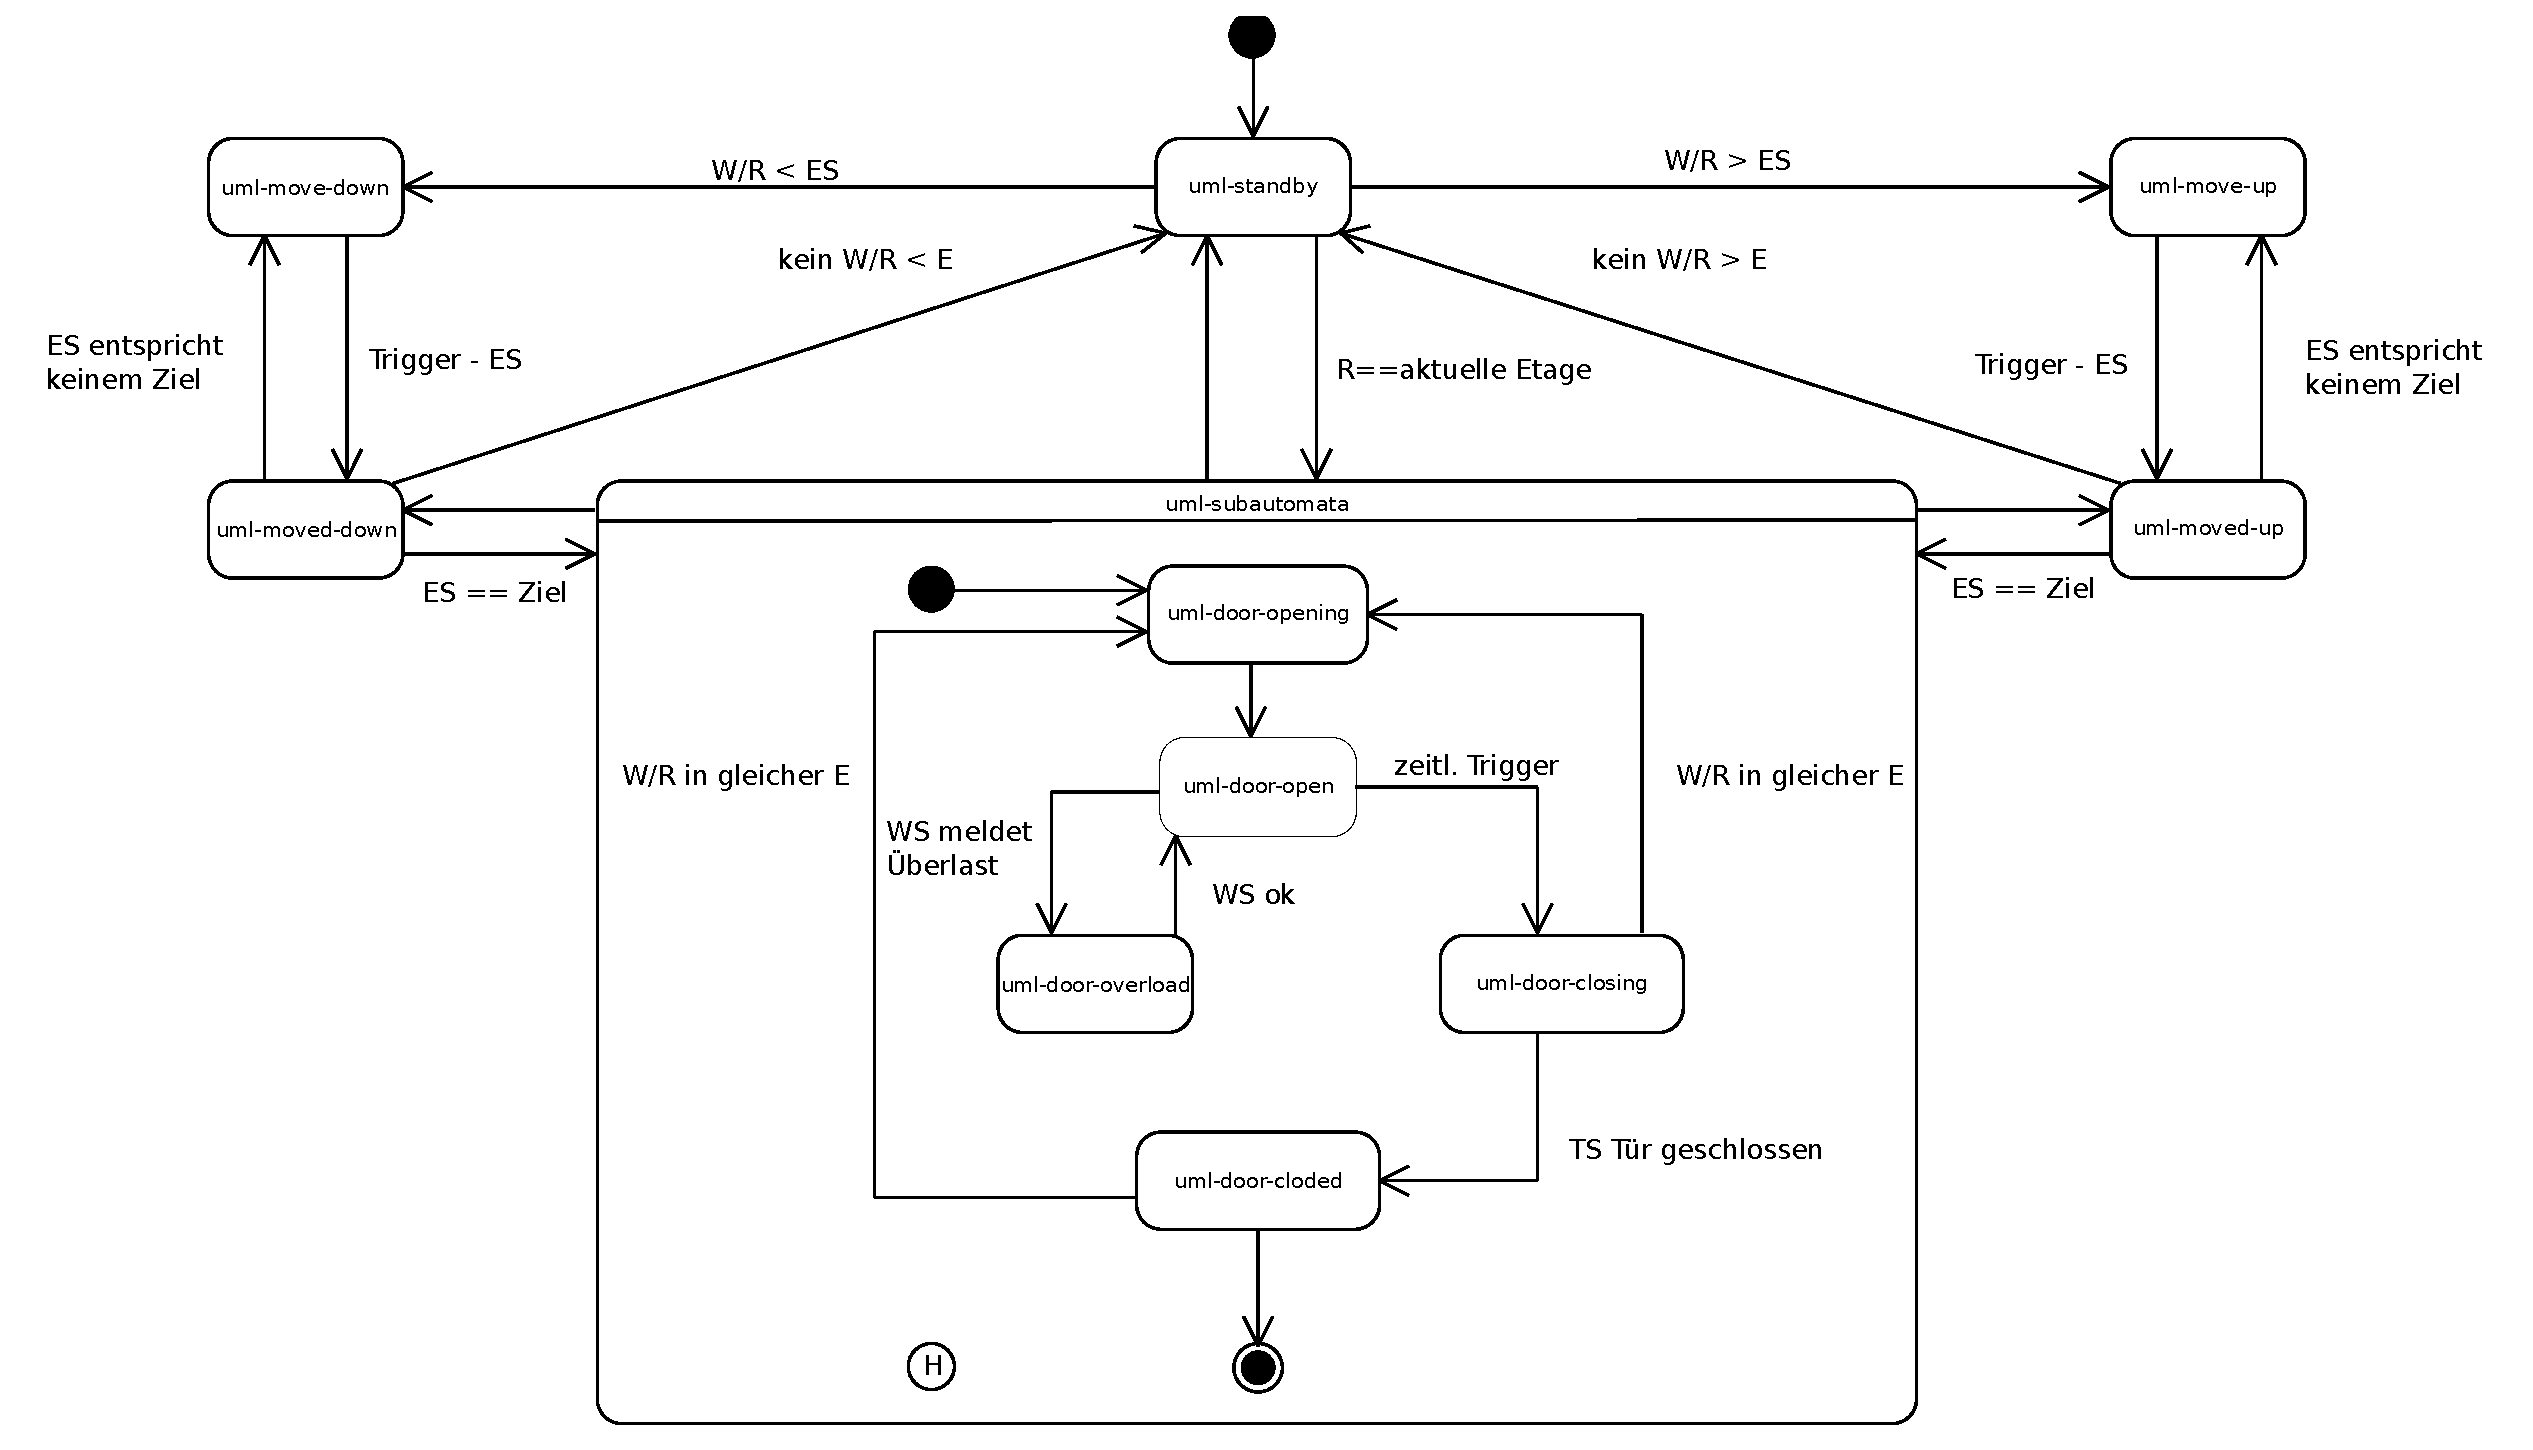
\includegraphics[width=1.3\textwidth]{images/ZDv6_id_view.eps}
	\caption{IDs des Zustandsdiagrammes}
	\label{fig:ZD_id_view}
\end{figure}

\newpage
\section{API}
\label{imp_api}
\begin{table}[h!]
	\begin{tabularx}{0.92\textwidth}{XX}
		\texttt{constructor(minLevel : Number, maxLevel : Number) : Elevator} & Konstruiert einen Elevator mit dem minimalen, bzw. maximalen Level \texttt{minLevel}, bzw. respektive \texttt{maxLevel}. \\ \hline
		\texttt{get minLevel() : Number}
		\texttt{get maxLevel() : Number}
		\texttt{get levelCount() : Number}
		\texttt{get level() : Number}
		\texttt{get direction() : Number}
		\texttt{get doorState() : String}
		\texttt{get isMoving() : Boolean}
		\texttt{get isDoorUnlocked() : Boolean}
		\texttt{get isOverweight() : Boolean}                             & Rudimentäre Getter um den Zustand des Elevator abzufragen. \\ \hline
		\texttt{addPerson() : void}                                       & Fügt dem Elevator eine simulierte Person hinzu. Der Elevator verfolgt nicht die Anzahl der Personen in ihm. \\ \hline
		\texttt{removePerson() : void}                                    & Entfernt vom Elevator eine simulierte Person. \\ \hline
		\texttt{hasRequest(level : Number, direction : Number) : Boolean} & Prüft ob auf der Etage \texttt{level} mit der Richtung \texttt{direction} ein Request vorliegt. Der Besondere Parameter \texttt{direction} wird in \textit{\nameref{imp_model}} näher beleuchtet. \\ \hline
		\texttt{request(level : Number, direction : Number) : void}       & Fügt dem Elevator ein Request für die Etage \texttt{level} mit der Richtung \texttt{direction} hinzu. Die möglichen Reaktionen des Elevator bei einem Aufruf werden in \textit{\nameref{imp_model}} näher beleuchtet. \\ \hline
	\end{tabularx}
\caption{Elevator}
\end{table}

\begin{table}[h!]
	\begin{tabularx}{0.92\textwidth}{XX}
		\texttt{constructor(elevator : Elevator) : ElevatorDoorSensor} & Konstruiert einen ElevatorDoorSensor und verbindet diesen mit einer Elevator Instanz. \\ \hline
		\texttt{get state() : String} & Gibt den aktuellen Zustand als String zurück: \textit{opening}, \textit{open}, \textit{shutting} oder \textit{shut}. \\ \hline
		\texttt{open() : void}        & Veranlasst eine Türöffnung, sofern der aktuelle Zustand den Übergang erlaubt. \\ \hline
	\end{tabularx}
\caption{ElevatorDoorSensor}
\end{table}

\begin{table}[h!]
	\begin{tabularx}{0.92\textwidth}{XX}
		\texttt{constructor(elevator : Elevator) : ElevatorWeightSensor} & Konstruiert einen ElevatorWeightSensor und verbindet diesen mit einer Elevator Instanz. \\ \hline
		\texttt{get weight() : Number} & Gibt das kummulierte Gesamtgewicht zurück welches der Sensor mittels \texttt{persons:add} und \texttt{persons:remove} ermittelt hat. \\ \hline
	\end{tabularx}
\caption{ElevatorWeightSensor}
\end{table}
	 

\part{Projektdokumentation}

\chapter{Anforderungs- und Problemanalyse}
Aufgabe der Anforderungsanalyse in diesem Projekt war es herauszufinden welches Problem die Kundin mit der zu entwickelnden Software lösen möchte. Dafür wurden Interviews mit dem Kunden durchgeführt und entsprechende Ergebnisse mit Hilfe von Audioaufzeichnung, Mitschriften und Fotografien protokolliert. Zur detaillierten Beschreibung einzelner Abläufe des Systems wurden Kreativtechniken wie das Zeichnen verschiedener Szenarien an einem Whiteboard sowie die manuelle Simulation des Fahrstuhles mit einem aus Pappe gefertigten Modells durchgeführt.
\begin{figure}[hbt]
\centering
\subcaptionbox{Skizze der Fahrstuhlsimulation am Whiteboard}[0.49\linewidth]
{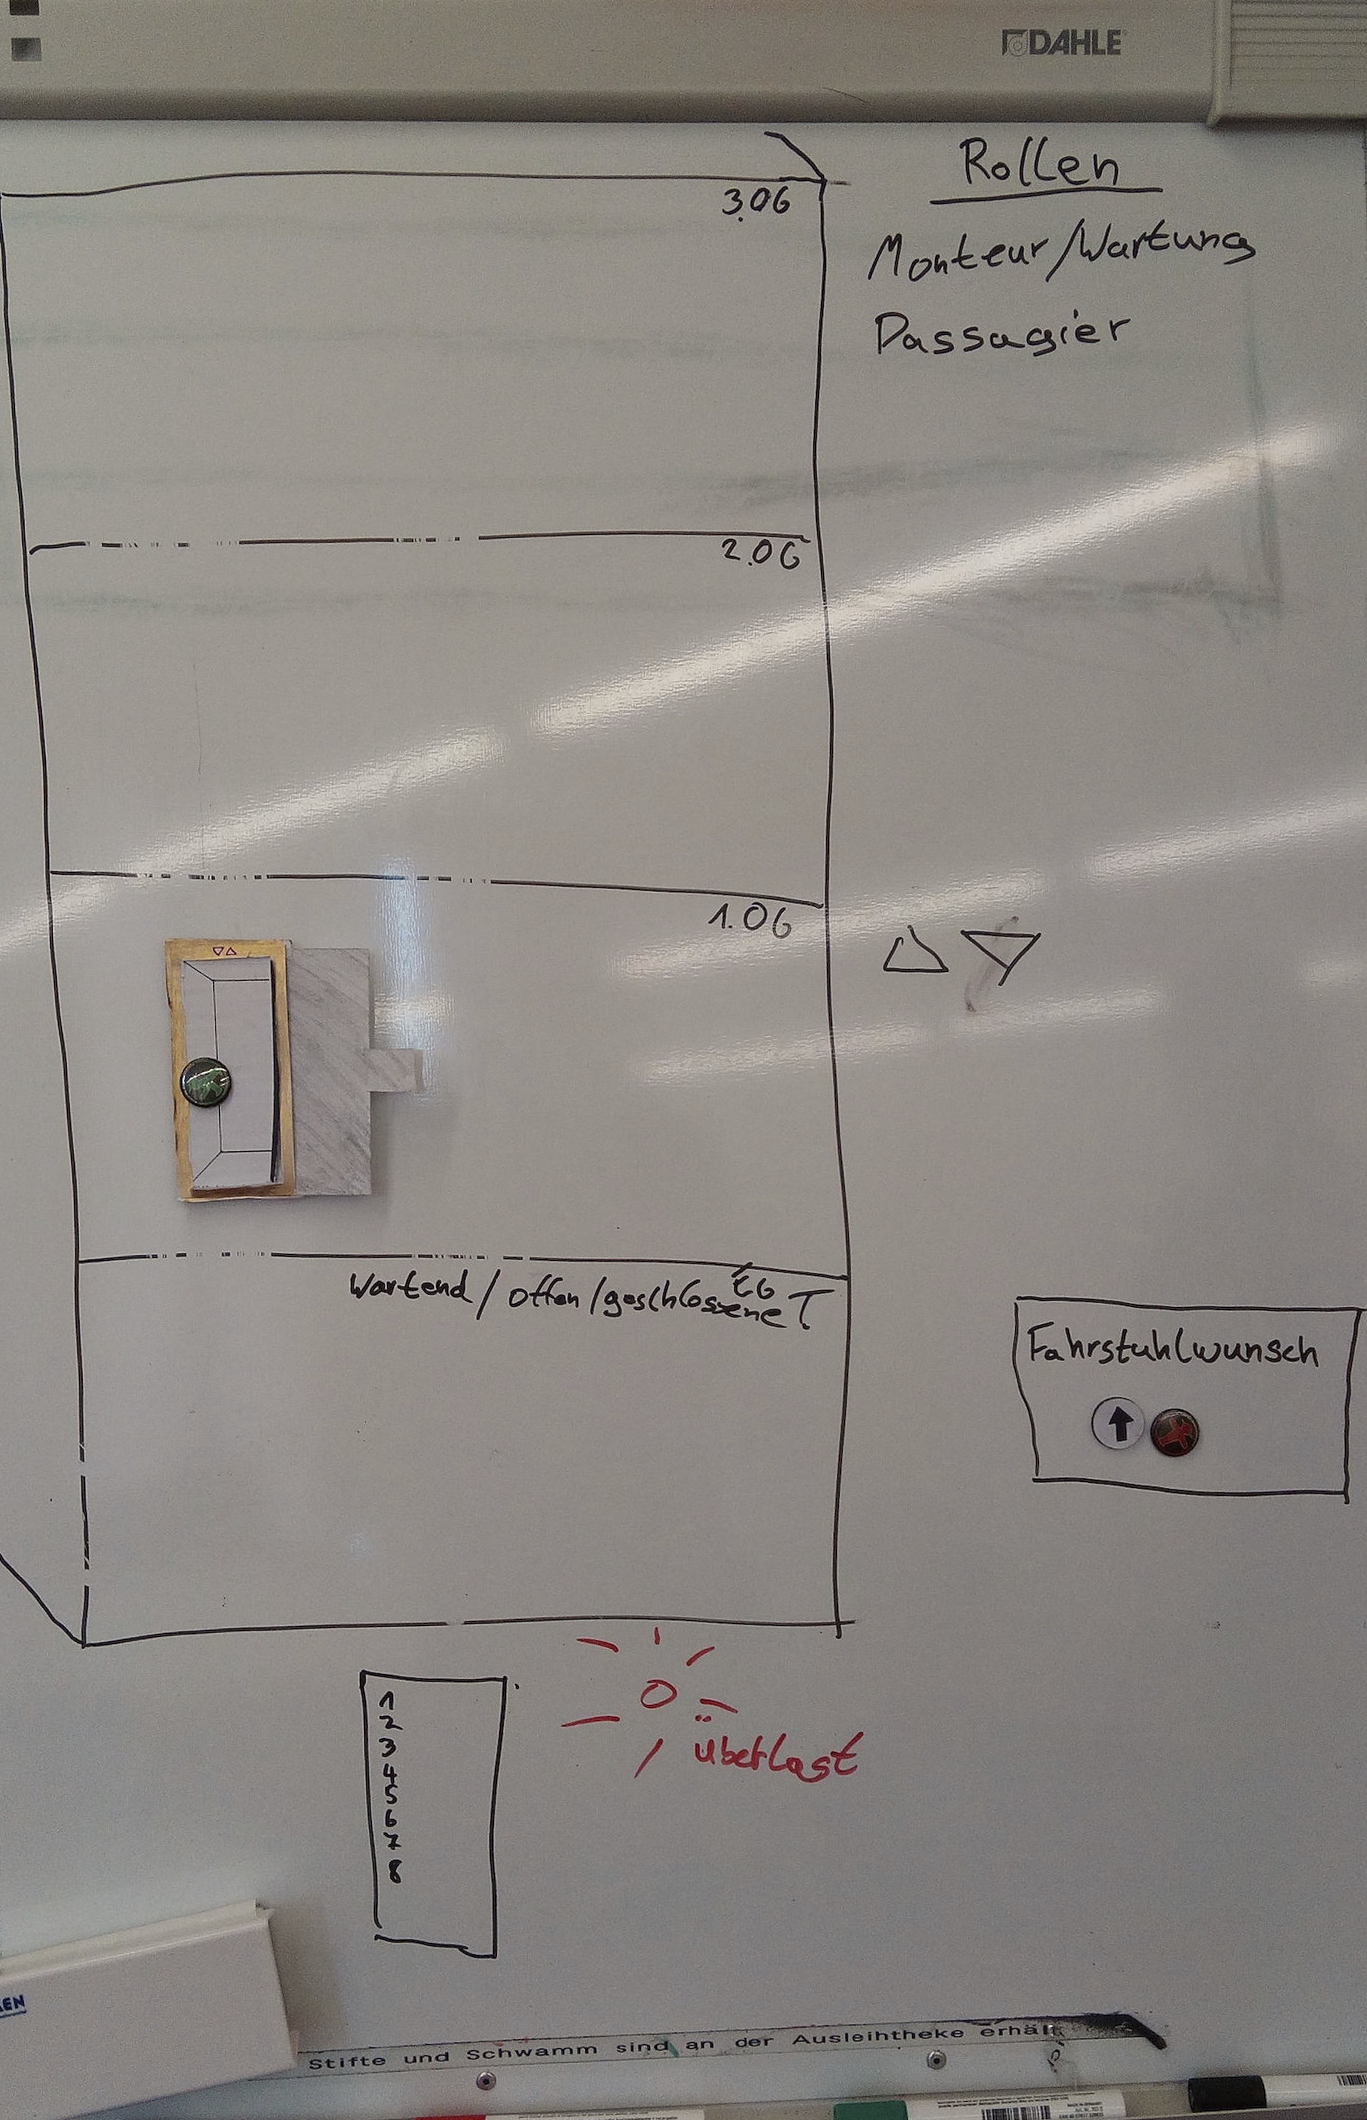
\includegraphics[height=8cm]{images/kundengespraech1.jpg}}
\subcaptionbox{Modell des Fahrstuhles}[0.49\linewidth]
{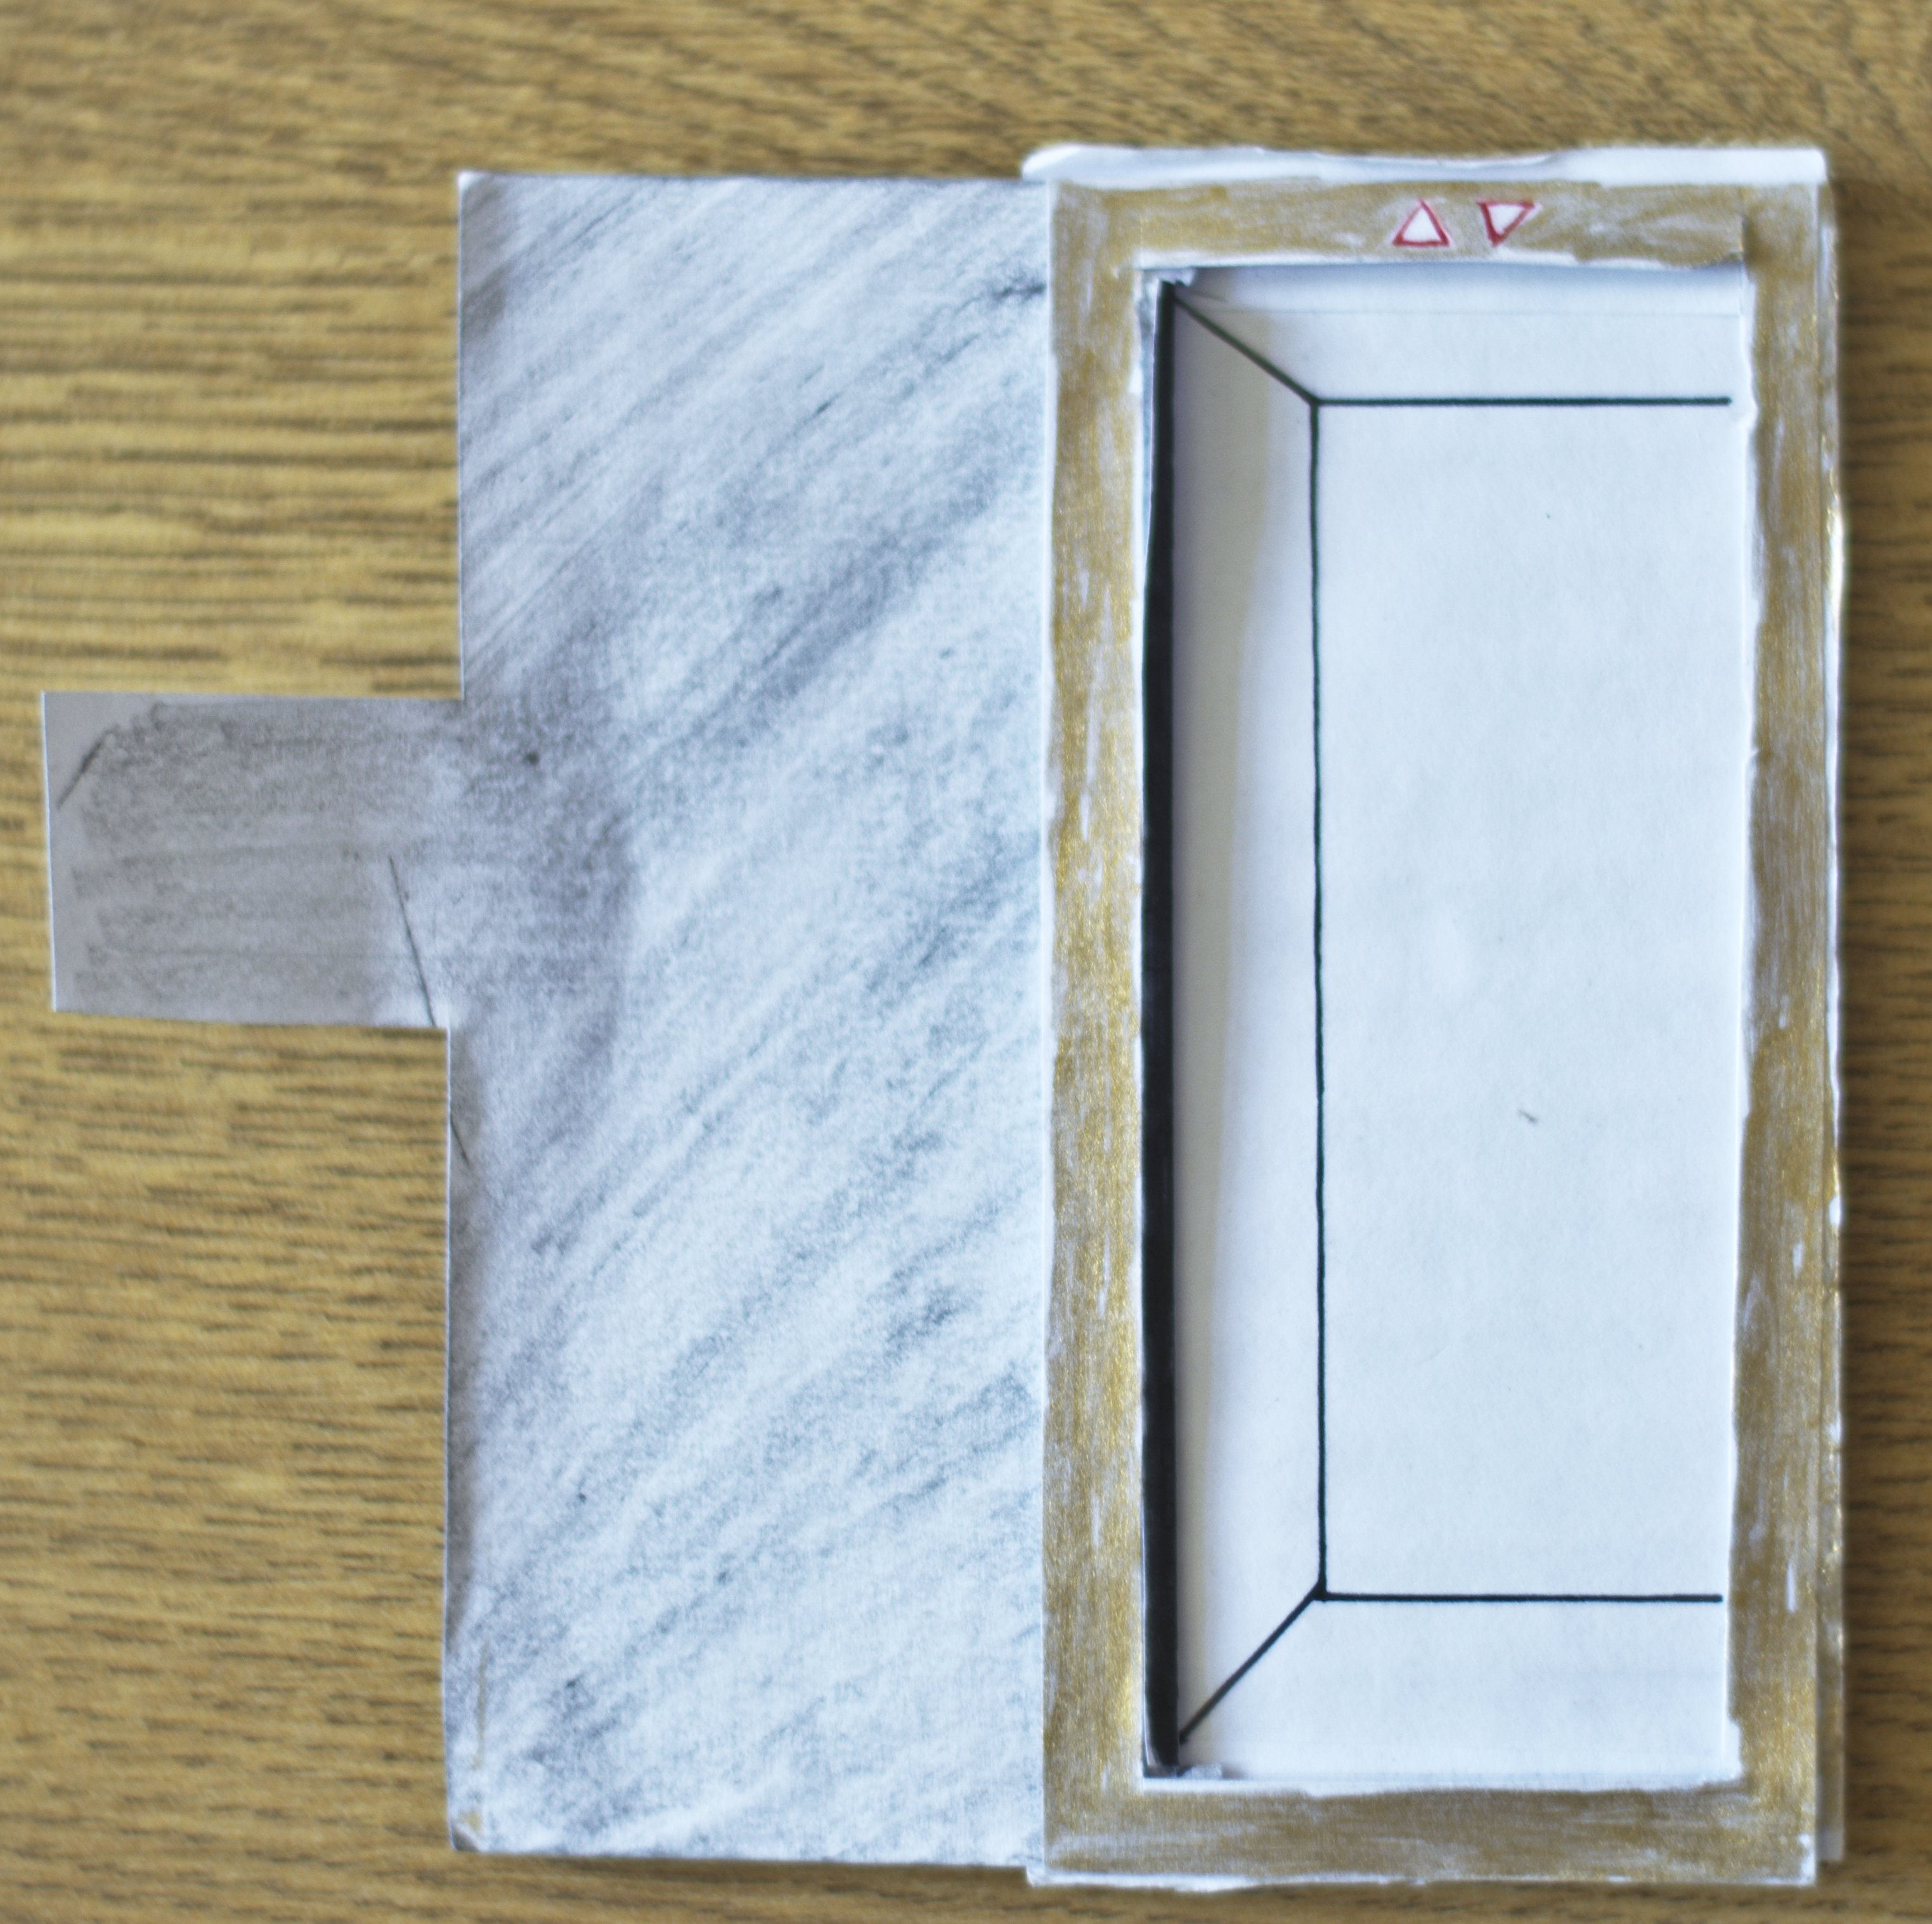
\includegraphics[height=8cm]{images/pappfahrstuhl.jpg}}
\caption{Kreativtechniken zur Anforderungsanalyse}
\end{figure}
Die folgenden grundlegende Fragen waren im Laufe der Analyse zu klären:
\begin{itemize}
	\item Wie viele Fahrstühle sollen verwendet werden können?
	\item Wie soll das Gebäude beschaffen sein?
	\item Welcher Algorithmus soll verwendet werden?
	\item Gibt es Schnittstellen zu anderen Systemen?
\end{itemize}
Weiterhin musste festgelegt werden ob die Priorität des Systems auf der Simulation oder auf einer möglichst realitätsnahen Umsetzung eines Liftes liegt. Im Laufe der Analyse und Modellierung entsprechender Anwendungsfälle wurde ersichtlich, dass das System sich aus zwei Teilsystemen, der \textbf{Fahrstuhlsteuerung} und der \textbf{Fahrstuhlsimulation} zusammensetzt, deren Anforderungen getrennt voneinander beschrieben werden mussten.\\
Eine Besonderheit des Systems ist dabei die Umgebung in der es eingesetzt werden soll, der Lehrbetrieb an einer Hochschule. Daraus ergaben sich spezielle Anforderungen, wie das Anzeigen der Zustandsübergänge, die gesondert betrachtet werden mussten.

\paragraph{}Vor allem aus den letztgenannten Anforderungen formte sich während der Analyse relativ früh unsere Vision einer Anwendung, welche in einer zweigeteilten Sicht Fahrstuhl und Zustandsdiagramm nebeneinander darstellt. Zusätzlich sollten Zustandsübergänge und aktive Zustände durch Animationen kenntlich gemacht werden.

\paragraph*{}Die Resultate der Analysephase, alle Anwendungsfälle und Vereinbarungen mit der Kundin wurden am Ende im Pflichtenheft festgehalten, welches als eigenständiges Dokument am Ende der Phase an die Kundin überreicht wurde. Diese Dokument war im weiteren Verlauf des Projektes ein zentrales Maß bei regelmäßigen Treffen und Evaluationen.



\chapter{Software-Entwurf}
Nach der Festlegung von Anforderungen und der Beschreibung der Funktionalitäten der Fahrstuhlsimulation war der nächste Schritt der Entwurf der internen Struktur. Wir näherten uns dieser Problemstellung von außen und erhöhten bei steigender Tiefe die Granularität. Dies bedeutete zunächst, die geeignetste Rahmen-Technologie festzulegen, welche die Anforderungen unseren Kundin am besten erfüllen konnte.

\section{Technologie}
Die Wahl der verwendeten Technologie fußte prinzipiell auf drei Hauptpunkten, erstens unserer Vision einer optisch ansprechenden Anwendung, welche das Zusammenspiel von System und dessen Zuständen visualisiert. Zweitens einer möglichst umfassenden Kompatibilität zu verschiedenen Plattformen und drittens der verfügbaren Zeit zur Realisierung aller Anforderungen. In Anbetracht der kurzen Projektzeit entschlossen wir uns zunächst eine Vorauswahl zu treffen. Diese sollte ausschließlich Technologien enthalten, auf deren Gebieten bereits Erfahrungen im Team vorhanden waren. Nach kurzer Diskussion ergaben sich als Möglichkeiten die Nutzung von \textsc{C++}, \textsc{Java} oder \textsc{Web-Technologien} wie \textsc{Javascript}.

\paragraph*{}Nach reiflicher Überlegung und wiederholter Rücksprache mit unserer Kundin erschienen uns \textsc{Web-Technologien} am geeignetsten um alle Anforderungen in der zur Verfügung stehenden Zeit umzusetzen. Die Vorteile dieser Technologien, welche unsere Entscheidung maßgeblich beeinflussten, waren folgende:

\begin{enumerate}
	\item Sie ermöglichten uns größtmögliche Plattform-Kompa\-tibilität, da unser Produkt einerseits als Cross-Plattfom-Anwendung und andererseits als Web-Site veröffentlicht werden können.
	\item Mit den modernen Mitteln des Web-Designs war es uns möglich die hohen grafischen Anforderungen an das Software-System in derart kurzer Zeit umzusetzen.
\end{enumerate}


\section{Algorithmus}
Die wesentliche Funktionalität sowie der Algorithmus des Systems lassen sich in
dem Zustandsdiagramm abbilden. Um das bestmögliche Ergebnis zu erhalten haben
wir verschiedene Versionen des Diagramms entworfen und diese in Gruppentreffen diskutiert und überarbeitet.
\missingfigure[figwidth=\textwidth]{Zustandsdiagramm ggf. mehrere Versionen}

\paragraph{}Diese Vorauswahl bestand
Für die technische Umsetzung der Zustände in ausführbaren Quellcode ergaben sich folgende Entwurfsmuster:
\todo{Wir müssen aufpassen, dass wir eine klare Trennung zwischen Entwurfs-spezifischen Inhalten im Entwicklerhandbuch und hier vornehmen.}
\subsection*{State Design Pattern}
Vorteile, Nachteile, warum haben wir uns dageben entschieden?
\todo{Nachteile: großer Overhead, da hier nur 3 Zustände vorkommen, jedoch die Zustandsübergänge komplex sind}
\subsection*{Zustandstabelle}
\todo{nicht sinnvoll zwecks erweiterbarkeit/wartbarkeit}

Die eigentliche Herausforderung des Systems besteht nicht in den Zuständen, sondern in den Zustandsübergängen, da der Fahrstuhl bis auf wenige Ausnahmen wie von \textbf{Idle} nach \textbf{Stop} in jeden beliebigen Zustand springen kann.
\subsection*{Event Emitter}
\subsection{Observer Pattern}

\chapter{Qualitätssicherung}
\section{Allgemein}
Der Standard ISO/IEC 25000:2014 welcher als Einleitung zu genormten Methoden der Qualitätssicherung in der Software zu verstehen ist, definiert diese als "`Systems and Software Quality Requirements and Evaluation (SQuaRE)"'\cite[Foreword]{ISO25000}. Festzustellen ist: Der ISO25000 ist für einen Norm relativ jung ist und löst zwei Vorgänger, welche die Themen Softwarequalität bzw. Anforderungsanalyse (ISO/IEC 9126) und Software Evaluierung bzw. Test (ISO/IEC 14598) überwiegend getrennt behandeln ab. Neben der Motivation der Vermeidung von Redundanzen und Inkonsistenzen zwischen den zwei Normen, ist es Meinung des Autors, dass sich hierbei die Erkenntniss der notwendigen Verzahnung der beiden Teilgebiete zeigt. So werden z.B. im \textit{test driven development} idealerweise die Anforderungen direkt zur Software-Evulation benutzt.

\paragraph*{}Aus der Definition
\begin{quote}\label{PD_SQ}
software quality
capability of software product to satisfy stated and implied needs when used unter specified condidtions
\end{quote}\cite[4 Terms and definitions]{ISO25000}
lässt sich somit die umfassende Qualitätssicherung aufteilen auf
\begin{enumerate}
\item Einwirkung auf Anforderungsanalyse
\item Evaluation während und nach der Umsetzung
\end{enumerate}
da sich Softwarequalität nach obiger Definition rein auf die bereits eruierten Anforderungen und Bedingungen stützt, wie Gesamtzufriedenheit des Nutzers allerdings nur dann erreichen lässt, wenn diese Vorbetrachtung bestmöglich durchgeführt wurde.
\section{QS Anforderungsanalyse}
Zu Beginn des Projekts wurde beim der Erstellung des Pflichtenheftes auf saubere und eindeutige Formulierungen geachtet, da Probleme in dieser Phase die größten Auswirkungen auf die Zufriedenheit des Nutzers besitzen.\\
Desweiteren wurde durch erneuten Vergleich der Anforderungen mit Kundenprotokollen und Aufgabenstellung sowie Prüfen auf Inkonsistenzen assistiert.

Als qualitätsunterstüzende Maßnahme wurden die Anforderungen möglichst auf sogenannte Issues, also Stichpunkte und Meilensteine in einem Projektmanager, abgebildet.
\section{QS Umsetzung}
\subsection{Allgemein}
\begin{itemize}
\item Konvetionen
\item Testregime
\end{itemize}
\subsection{Konventionen}
\todo{Traceabillity hinzufügen -> jede Anforderung muss im Quellcode durch einen commit oder ähnlich nachverfolgbar sein}
\subsection{Codekonventionen}
Um bei der Arbeit in der Gruppe an einer gemeinsamen Quellcode-Basis einen hohen Qualitätsstandard der Quelltexte zu bewahren, wurden Konventionen festgelegt die den Entwicklern vorgeschrieben haben wie z.B. Methoden und Variablen benannt werden sollen. So wurde festgelegt, dass
\begin{itemize}
 \item Methodennamen in camelCase Notation zu bezeichnen sind
 \item im Quelltext keine nachgestellten Leerzeichen\footnote{engl. trailing whitespace} vorkommen dürfen
 \item keine Quelltextzeile länger als 80 Zeichen ist
 \item private Variablen mit einem Unterstrich gekennzeichnet werden
\end{itemize}

\todo{Code Konventionen, statische Codeanalyse}
\subsection{Test}
Für die automatischen Tests wurde das Testframework Jasmine\footnote{http://jasmine.github.io}

\subsubsection{manuelle Testfälle}
\subsubsection{automatisierte Testfälle}

\chapter{Team-Organisation}
\section{Gruppenarbeit}
Um das Zusammenarbeiten in der Gruppe einfacher zu gestalten wurden verschiedene Technologien eingesetzt.
Zu finden von Terminen für Meetings wurde Doodle\footnote{\url{www.doodle.com}}  verwendet. Für die Kommunikation in der Gruppe Slack\footnote{\url{https://slack.com/}}.
\todo{Hier muss hin warum wir uns für JS und Co entschieden haben.}
\section{Verwendete Werkzeuge}
\section{Resümee}

\bibliographystyle{plaindin}
\bibliography{projektdokumentation}


\chapter{Glossar}
\glsaddall % bindet auch nicht verwendete Glossareinträge ein
\nocite{*} % zeige auch nicht zitierte Einträge des Literaturverzeichnisses
\glossarystyle{altlist} % erzeugt Zeilenumbruch nach dem Name des Elements
\printglossary[title=Allgemeiner Glossar, toctitle=Allgemeiner Glossar, type=allg]
\printglossary[title=Projektspezifischer Glossar, toctitle=Projektspezifischer Glossar]
%\printglossary[title=Abk"urzungen, type=\acronymtype]
\end{document}